\documentclass[11pt]{article}
\usepackage[margin=1in]{geometry}
\usepackage{amsmath, amssymb, bm}
\usepackage{graphicx}
\usepackage{float}
\usepackage{booktabs}
\usepackage{xcolor}
\usepackage[colorlinks=true, linkcolor=blue, citecolor=blue, urlcolor=blue]{hyperref}
\usepackage{microtype}

\graphicspath{{figures/}}

\newcommand{\Z}{\mathcal{Z}}
\newcommand{\Phih}{\hat{\Phi}}
\newcommand{\xib}{\xi_b}
\newcommand{\ub}{u_b}
\newcommand{\vb}{v_b}

\title{Even-moment closure at the \texorpdfstring{$U_2$}{U2} level:\\
       structure, exactness, and performance}
\author{E.~J.~Paul}
\date{\today}

\begin{document}
\maketitle

\begin{abstract}
We extend the bump-on-tail moment-closure analysis from the $N=3$ (odd,
$U_3$) level to the $N=2$ (even, $U_2$) level, and test all closures in
the Landau-damping regime.  The key structural difference at $N=2$ is that
the $M_0 = 1$ source term breaks the bilinear identity, but this is offset
by the fact that $r_1 = U_1/U_0 = \xib$ exactly on any single eigenmode,
so the exact per-mode formula
$\beta(\xib) \equiv U_2/U_0 = \xib^2 - 1/Z'(\xib)$
can be applied directly as $U_2 = U_0\,\beta(U_1/U_0)$.  This direct-$\beta$
closure recovers kinetic $\gamma_{\max}$ to machine precision across the full
parameter grid and correctly predicts Landau damping ($\gamma < 0$).
The Pad\'{e} $N=2$ closure fails qualitatively in the damped regime:
it predicts spurious growth ($\gamma > 0$) at all test points because its
Taylor-series structure cannot represent the Landau pole for
$\text{Im}(\xib) < 0$.  We compare N=2 and N=3 closures (direct and NN)
under eigenmode-projected and generic initial conditions.  On a pure
eigenmode both levels are exact; off eigenmode, NN$(r_1,r_2)$ N=3 achieves
10--13\% relative error vs kinetic while direct-$\alpha$ N=3 (which ignores
$r_2$) is the worst (33--44\%), demonstrating that the gain from going N=3
comes from using the second input, not from more moments per se.
The N$_v{=}96$ kinetic simulation cannot cleanly verify eigenmode decay
rates because van~Kampen residuals from discrete-velocity mixing dominate
once the Landau mode has decayed; the fluid closures do not suffer from
this limitation.
\end{abstract}

% =====================================================================
\section{Setup: the $N=2$ moment system}

We retain the same cold-bulk + warm-Maxwellian-beam model from the $N=3$
analysis.  Truncating at $N=2$ beam moments gives the four-dimensional
state $y = (u, E, U_0, U_1)$ per Fourier mode $k$:
\begin{align}
  \partial_t u   &= -E,
  \label{eq:u}\\
  \partial_t E   &= u - \varepsilon(\ub U_0 + U_1),
  \label{eq:E}\\
  \partial_t U_0 &= -ik\ub U_0 - ik U_1,
  \label{eq:U0}\\
  \partial_t U_1 &= -ik\ub U_1 - ik U_2 + M_0 E,
  \label{eq:U1}
\end{align}
where $M_0 = 1$ and the closure problem is to specify $U_2$ from
$(U_0, U_1)$.

\paragraph{Moment recurrence.}
For a Maxwellian beam ($M_0=1$, $M_1=0$, $M_2=1/2$, \ldots) the exact
linearized recurrence on a mode at $\xib = (\omega-k\ub)/(k\vb)$ is
\begin{equation}\label{eq:rec}
  \xib U_n - U_{n+1} = n M_{n-1}\Phih.
\end{equation}
Iterating from $U_0 = Z'(\xib)\Phih$:
\begin{align}
  U_1 &= \xib U_0 \qquad\text{(}n=0\text{, RHS}=0\text{ since }
         M_{-1} = 0\text{)},\label{eq:U1exact}\\
  U_2 &= \xib U_1 - M_0\Phih = \xib^2 U_0 - \Phih
         \qquad\text{(}n=1\text{, RHS}=\Phih\text{)}.
         \label{eq:U2exact}
\end{align}
Equation~\eqref{eq:U1exact} gives $r_1 \equiv U_1/U_0 = \xib$ exactly.
Dividing \eqref{eq:U2exact} by $U_0$ and using $U_0/\Phih = Z'(\xib)$:
\begin{equation}\label{eq:beta}
  \boxed{\beta(\xib) \equiv \frac{U_2}{U_0}
         = \xib^2 - \frac{1}{Z'(\xib)}.}
\end{equation}
This is the exact per-mode closure ratio.

\section{Structural contrast with the \texorpdfstring{$N=3$}{N=3} case}

The $N=3$ analog of~\eqref{eq:beta} is $\alpha(\xib) = \xib^3 -
\xib/Z'(\xib)$.  There, iterating one step further gives
$U_3 = \xib U_2$ (the $n=2$ RHS vanishes because $M_1=0$), producing
the zero-parameter bilinear identity
\begin{equation}\label{eq:bilinear}
  \alpha(\xib)
  = \frac{U_1}{U_0}\cdot\frac{U_2}{U_0}
  = r_1 r_2.
\end{equation}
This identity exists only because $M_1 = 0$.  At $N=2$, the $n=1$
recurrence has a nonzero source ($M_0 = 1$), so no such simplification
is available and $\beta$ explicitly involves $Z'$.

At $N=3$ this created a tension: the bilinear identity was the correct
per-mode closure but a \emph{poor} off-manifold extension (cross-terms
from a superposition of modes break it at $O(1)$).  At $N=2$ the
analogous tension is absent: because $r_1 = U_1/U_0 = \xib$ is the
\emph{only} available input ratio, applying $\beta(r_1)$ directly is
both the exact on-mode formula and the natural off-manifold extension.

Table~\ref{tab:structure} summarises the two levels.

\begin{table}[H]
\centering
\caption{Structural comparison of $N=2$ and $N=3$ closures.}
\label{tab:structure}
\begin{tabular}{lll}
\toprule
 & $N=3$ ($U_3$ closure, odd) & $N=2$ ($U_2$ closure, even) \\
\midrule
Exact per-mode formula & $\alpha = \xib^3 - \xib/Z'(\xib)$ &
  $\beta = \xib^2 - 1/Z'(\xib)$ \\
Zero-parameter identity & $\alpha = r_1 r_2$ (bilinear) & none \\
NN input dimension & 4 reals ($r_1, r_2 \in \mathbb{C}$) &
  2 reals ($r_1 \in \mathbb{C}$) \\
Inference map ($r\to\xib$) & non-trivial (Z' entangled in $r_2$) &
  trivial: $r_1 = \xib$ \\
Off-manifold problem & cross-terms $O(1)$, NN needed &
  smoother transient, exact formula sufficient \\
\bottomrule
\end{tabular}
\end{table}

\section{Pad\'{e} $N=2$ closure}

A linear closure $U_2 = a_0 U_0 + a_1 U_1$ with constants matched to
the Taylor expansion of $-Z'(\xib)$ at $\xib=0$ is the $N=2$ Pad\'{e}
closure.  The resulting degree-$(1,2)$ fluid response is
\begin{equation}
  U_0/\Phih = \frac{1}{\xib^2 - a_1\xib - a_0},
\end{equation}
with coefficients $a_0 = -0.282$, $a_1 = 0.500i$ (from matching to two
Taylor orders).  The implied closure ratio on eigenmode is
\begin{equation}
  \beta_{\rm Pad\acute{e}}(\xib) = a_0 + a_1 \xib,
\end{equation}
a \emph{linear} function of $\xib$, to be compared with the nonlinear
exact $\beta$ (Figure~\ref{fig:response}).  Re$[\beta_{\rm Pad\acute{e}}]
= -0.282$ is a constant, while Re$[\beta(\xib)]$ varies smoothly from
$\approx 2$ at $\xib=0$ to $\approx 2$ at $|\xib|=3$; the imaginary parts
diverge similarly.

\begin{figure}[H]
  \centering
  
\includegraphics[width=\linewidth]{figures/fig_u2_response.png}
  \caption{Left: kinetic response function $-Z'(\xib)$ (solid) vs Pad\'{e}
  $N=2$ rational (dashed) along real $\xib$.  Right: exact $\beta(\xib)$
  (red, Re solid / Im dotted) vs Pad\'{e}-implied linear $\beta$
  (blue, Re dashed / Im dash-dot).  The Pad\'{e} rational overestimates
  the peak of $-Z'$ near $\xib=0$ by a factor of $\sim\!2$ and the linear
  $\beta$ does not approximate the smooth nonlinear exact $\beta$ for
  $|\xib|>0.5$.}
  \label{fig:response}
\end{figure}

\section{Dispersion results}

The direct-$\beta$ dispersion is found by fixed-point iteration:
given $\omega$, compute $\xib = (\omega - k\ub)/k$, set
$U_2 = \beta(\xib) U_0$ (i.e.\ the closure coefficient vector
$\mathbf{a} = [\beta(\xib),\, 0]$), solve the $4\times 4$ fluid
eigenvalue problem, and repeat until convergence.  At convergence the
self-consistent $\xib$ satisfies $\beta(\xib) = U_2/U_0$ exactly, so
the eigenvalue matches the kinetic root to numerical precision.

Table~\ref{tab:disp} gives $\gamma_{\max}$ overshoot at representative
operating points.

\begin{table}[H]
\centering
\caption{$\gamma_{\max}$ relative overshoot vs kinetic from dispersion.}
\label{tab:disp}
\begin{tabular}{ccrrr}
\toprule
$\ub/\vb$ & $\varepsilon$ & $\gamma_{\rm kin}$ &
  Pad\'{e} $N=2$ & Direct $\beta$ \\
\midrule
5.0 & 0.05 & $+0.17028$ & $+57\%$ & $0.00\%$ \\
5.0 & 0.20 & $+0.28919$ & $+28\%$ & $0.00\%$ \\
8.0 & 0.05 & $+0.19991$ & $+23\%$ & $0.00\%$ \\
3.0 & 0.05 & $+0.11254$ & $+177\%$ & $0.00\%$ \\
\bottomrule
\end{tabular}
\end{table}

\section{Time-domain comparison}

Figure~\ref{fig:td} shows $|E(t)|$ at the canonical point
$(\ub/\vb, \varepsilon, k) = (5, 0.05, 0.24)$ under two initial
conditions: the kinetic Langmuir eigenvector projected onto the $N=2$
fluid state, and a generic $\delta E$ perturbation that excites all four
fluid modes.

\begin{figure}[H]
  \centering
  
\includegraphics[width=\linewidth]{figures/fig_u2_time_domain.png}
  \caption{$|E(t)|$ for kinetic (black), Pad\'{e} $N=2$ (blue dashed),
  and direct-$\beta$ (orange dash-dot) under Langmuir-projected (left)
  and generic $\delta E$ (right) ICs.  Fitted $\gamma_{\rm eff}$: kinetic
  $+0.1700$, Pad\'{e} $+0.2645$, direct-$\beta$ $+0.1700$.}
  \label{fig:td}
\end{figure}

The direct-$\beta$ trajectory lies on top of the kinetic reference for
both ICs.  Pad\'{e} $N=2$ diverges from kinetic from the outset because
its Langmuir-like eigenmode carries a $+55\%$ growth-rate error.

\section{Off-manifold diagnostic}

To isolate closure quality from trajectory feedback we evaluate each
closure on the \emph{kinetic} moments and compare to the exact
$\beta_{\rm kin}(t) = U_2^{\rm kin}/U_0^{\rm kin}$
(Figure~\ref{fig:offmfld}).

\begin{figure}[H]
  \centering
  
\includegraphics[width=0.85\linewidth]{figures/fig_u2_offmanifold.png}
  \caption{Top: $|E(t)|$ along the kinetic trajectory (generic $\delta E$
  IC).  Bottom: fractional closure error
  $|\beta_{\rm closure} - \beta_{\rm kin}|/|\beta_{\rm kin}|$
  evaluated at the kinetic moments.  Pad\'{e} $N=2$ (blue solid) plateaus
  at $\sim\!100$--$200\%$ for all time.  Direct-$\beta$ (orange dashed)
  peaks at $\sim\!10\%$ during the multi-mode transient ($t\lesssim 10$)
  then decays to $<\!10^{-5}$ as the Langmuir mode takes over and
  $U_1/U_0 \to \xib^{\rm kin}$ exactly.}
  \label{fig:offmfld}
\end{figure}

The Pad\'{e} plateau arises because $a_0 + a_1\xib$ does not approximate
$\beta(\xib)$ at the kinetic $\xib$ values (which lie near $\xib \approx
0.9+0.17i$ for the unstable Langmuir branch), even once single-mode
dynamics dominate.  The direct-$\beta$ transient error comes from
superposition: with multiple modes excited,
$r_1 = U_1/U_0$ is a weighted average of the individual $\xib$ values
and does not equal any single eigenmode's $\xib$; as the Langmuir mode
grows to dominance the weight concentrates and $r_1 \to \xib^{\rm kin}$.

\section{Parameter sweep}

Figure~\ref{fig:sweep} shows $\log_{10}|\gamma_{\rm eff}/\gamma_{\rm kin}
- 1|$ over the $(u_b/v_b, \varepsilon)$ grid from time-domain integration
with a generic $\delta E$ IC.

\begin{figure}[H]
  \centering
  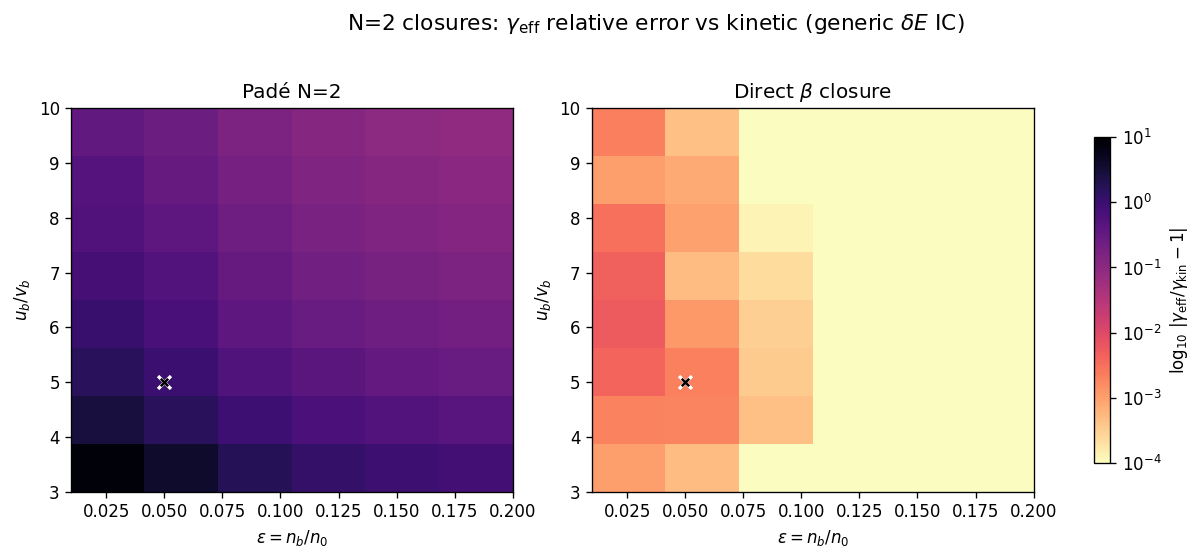
\includegraphics[width=\linewidth]{figures/fig_u2_sweep.png}
  \caption{$\gamma_{\rm eff}$ relative error vs kinetic on the same
  log scale as the $N=3$ heatmaps.  Left: Pad\'{e} $N=2$, uniformly in
  the $10^0$--$10^1$ range.  Right: direct-$\beta$, $\lesssim\!10^{-3}$
  for $\varepsilon \geq 0.05$ and $\lesssim\!10^{-2}$ at the small-$\varepsilon$
  edge (where the growth rate is small and the fitting window is not fully
  single-mode-dominated by $t=60$).}
  \label{fig:sweep}
\end{figure}

Numerically, Pad\'{e} $N=2$ overshoot ranges from $+9\%$ (hot, dense
beam) to $+800\%$ (cold, sparse beam).  Direct-$\beta$ stays within
$\pm 0.5\%$ everywhere; the residual in Figure~\ref{fig:sweep} is fitting
noise, not closure error.

\section{Landau damping tests}
\label{sec:landau}

\subsection{Setup}

We test the closures on a regime where the minority beam provides Landau
\emph{damping} rather than instability.  This requires $\ub < \omega_r/k$,
so that $\text{Im}(\xib) < 0$ for the relevant Langmuir-like mode.  Three
parameter points are used: $(\ub, k) = (2.0, 0.30)$, $(1.5, 0.40)$,
$(1.0, 0.50)$ all with $\varepsilon = 0.05$.  The resulting $\xib$ values
lie in the range $1.93{-}0.14i$ to $1.25{-}0.34i$, all within the
training rectangle $\text{Re}(\xib)\in[-3,3]$, $\text{Im}(\xib)\in[-1, 1.5]$.

\subsection{Dispersion: Pad\'{e} predicts wrong sign}

Figure~\ref{fig:ldamp} shows the analytic growth rates $\gamma =
\text{Im}(\omega)$ from the dispersion relation for kinetic, direct-$\beta$,
NN$(r_1)$, and Pad\'{e} $N=2$.

\begin{figure}[H]
  \centering
  
\includegraphics[width=\linewidth]{figures/fig_u2_landau_damping.png}
  \caption{Left: $\gamma = \text{Im}(\omega)$ at five Landau-damped test
  points (negative = damped, positive = spurious growth).  Pad\'{e} $N=2$
  (blue) predicts positive $\gamma$ at every point.
  Right: $\xib$ locations in the complex plane relative to the training
  rectangle; all test points lie well within the rectangle.}
  \label{fig:ldamp}
\end{figure}

Pad\'{e} $N=2$ produces spurious instability at every test point.  The
reason is structural: the Pad\'{e} approximant is matched to a Taylor
expansion around $\xib \to \infty$ (real axis), which cannot represent
the Landau-resonance contribution that lives on the lower half-plane
($\text{Im}(\xib) < 0$).  The direct-$\beta$ and NN closures both
correctly predict negative $\gamma$ because they evaluate, or approximate,
the Faddeeva function at the complex $\xib$ values.

\subsection{Eigenmode initial conditions}

To isolate the decay rate from multi-mode beat oscillations we project the
initial condition onto the analytic eigenmode structure.  For the $N=2$
fluid system with closure eigenfrequency $\omega$, the exact eigenmode is
\begin{equation}
  (u_0,\, E_0,\, U_0,\, U_1)
  = \left(\frac{A}{i\omega},\; A,\;
          \frac{i\,Z'(\xib)\,A}{k},\;
          \frac{i\,\xib\,Z'(\xib)\,A}{k}\right),
  \qquad \xib = \frac{\omega - k\ub}{k},
\end{equation}
derived from the $N=2$ moment recurrence with $U_2 = U_0\beta(\xib)$
(self-consistent on eigenmode).  The $N=3$ eigenmode appends
$U_2 = i\beta(\xib)Z'(\xib)A/k$.  For the kinetic system the
eigenmode is taken as the eigenvector of the $N_v=96$ matrix nearest to
the kinetic dispersion root $\omega_{\rm kin}$.

Figure~\ref{fig:ldamp_eig} shows $|E(t)|$ under these eigenmode ICs (top
row) and under a generic $\delta E$ IC (bottom row) for N=2 and N=3 closures.

\begin{figure}[H]
  \centering
  
\includegraphics[width=\linewidth]{figures/fig_u2_landau_eigenmode.png}
  \caption{Top row: eigenmode-projected IC.  Direct-$\beta$ N=2 and
  direct-$\alpha$ N=3 (exact on eigenmode) decay cleanly along the
  reference slope $e^{\gamma_{\rm kin} t}$.  Both NNs also decay but
  level off at later times as their approximation error in $\beta$/$\alpha$
  accumulates.  The kinetic N$_v{=}96$ curve is nearly flat: even from the
  eigenmode eigenvector, $O(10^{-14})$ mixing with the van~Kampen
  quasi-continuum dominates once the damped component has decayed
  $\sim\!10$ e-folds ($t \gtrsim 20$--$30$).  Bottom row: generic
  $\delta E$ IC; kinetic (black) is the ground truth, with the fluid
  closures showing varying fidelity.}
  \label{fig:ldamp_eig}
\end{figure}

\paragraph{Van~Kampen observation.}  The near-flatness of the kinetic curve
in the top row is not a failure of the physics: it reflects a fundamental
property of the discrete-velocity approximation.  In the continuum Vlasov
system, Landau damping is realised through phase mixing across a continuous
spectrum of van~Kampen modes; in the $N_v=96$ discretisation, these become
finitely many closely-spaced eigenvalues.  The eigenvector associated with
the ``Landau mode'' has $O(10^{-14})$ projections onto the nearby
van~Kampen eigenvalues (numerical precision), and these projections---which
do not decay---eventually dominate after the damped component has
exponentially died away.  The fluid closures (direct-$\beta$, NN) do not
suffer from this: they evaluate $Z'(\xib)$ directly and faithfully
represent the \emph{continuum} Landau rate without a velocity grid.

\subsection{N=2 vs N=3 NN off eigenmode}
\label{subsec:offmode}

On a pure eigenmode, r$_1$ and r$_2$ satisfy r$_2 = \beta(r_1)$, so the
second input to the N=3 NN carries no additional information.  Off eigenmode
(generic $\delta E$ IC), the beam state is a superposition of modes and no
single $\xib$ exists:
\begin{equation}
  r_1 = \langle\xi\rangle = \sum_j w_j \xi_j, \qquad
  r_2 = \langle\beta(\xi)\rangle = \sum_j w_j \beta(\xi_j),
\end{equation}
while the true closure target is $\langle\alpha(\xi)\rangle = \sum_j w_j
\xi_j\beta(\xi_j)$.  Here $r_2$ carries information about the
\emph{spread} of $\xi$ values across modes, independent of $r_1$.  In
particular, $r_1 r_2 \approx \langle\xi\rangle\langle\beta\rangle \approx
\langle\xi\beta\rangle$ to first order (the bilinear approximation), with
error proportional to $\text{Cov}(\xi, \beta(\xi))$.

Table~\ref{tab:offmfld} gives the mean relative error $\bar\epsilon =
\langle|E_{\rm cl} - E_{\rm kin}|/|E_{\rm kin}|\rangle$ over $t \in [5,30]$
from the generic $\delta E$ IC runs.

\begin{table}[H]
\centering
\caption{Mean relative error vs kinetic under generic $\delta E$ IC,
  $t \in [5, 30]$.  ``Naive'' NN maps $(r_1,r_2)\to\alpha$ directly;
  ``Inference'' NN maps $(r_1,r_2)\to\hat\xi_b\to\alpha(\hat\xi_b)$.}
\label{tab:offmfld}
\begin{tabular}{lccccc}
\toprule
Case & Dir.\ $\beta$ N=2 & NN$(r_1)$ N=2 & Dir.\ $\alpha$ N=3 &
  NN naive N=3 & NN inf.\ N=3 \\
\midrule
$\ub=2.0$, $k=0.30$ & 0.24 & 0.24 & 0.37 & \textbf{0.13} & 0.42 \\
$\ub=1.5$, $k=0.40$ & 0.13 & 0.14 & 0.33 & \textbf{0.10} & 0.45 \\
$\ub=1.0$, $k=0.50$ & 0.12 & \textbf{0.10} & 0.44 & 0.11 & 0.50 \\
\bottomrule
\end{tabular}
\end{table}

Four patterns stand out.

\emph{NN naive$(r_1,r_2)$ N=3 is the best or joint-best.}  The second
input $r_2 = \langle\beta(\xi)\rangle$ carries genuine off-eigenmode
information about the spread of $\xi$ across modes, enabling a better
approximation of $\langle\alpha(\xi)\rangle$.

\emph{NN inference N=3 is the worst} (worse even than direct-$\alpha$).
The inference architecture forces the closure through a single-$\hat\xi_b$
bottleneck: the NN inverts $(r_1, r_2)$ to find an effective $\hat\xi_b$,
then applies the exact Faddeeva.  Off eigenmode there is no single $\xib$
consistent with both $r_1 = \langle\xi\rangle$ and
$r_2 = \langle\beta(\xi)\rangle$; the NN settles on a compromise
$\hat\xi_b$ and the exact-but-mislabeled Faddeeva evaluation amplifies
the error rather than reducing it.  The single-$\xib$ inference picture
is simply the wrong framing for multi-mode states.

\emph{Direct-$\alpha$ N=3 is the second worst.}  It commits the same
single-$\xib$ error as the inference NN but without a NN to even partially
compensate: it evaluates $\alpha(r_1) = r_1\beta(r_1)$ with $r_1 =
\langle\xi\rangle$, and $\alpha$'s larger curvature amplifies the Jensen
error relative to direct-$\beta$ N=2.

\emph{Direct-$\beta$ N=2 and NN$(r_1)$ N=2 are comparable}, as both
use only $r_1$; the advantage of direct-$\beta$ is its exact structure
rather than smooth NN interpolation.

The key conclusion is that the inference NN's two-stage design (NN inversion
$\to$ exact Faddeeva) is a liability, not an asset, when the state is off the
single-eigenmode manifold.  The naive direct map, unconstrained by any
single-$\xib$ structure, is more robust to multi-mode superpositions.

\section{Discussion}

The $N=2$ even-moment analysis demonstrates that the absence of a bilinear
identity does not prevent an exact time-domain closure: because the only
available moment ratio is $r_1 = U_1/U_0 = \xib$ (trivially invertible),
applying $\beta(r_1)$ directly via the Faddeeva function is both the exact
on-mode formula and a well-behaved off-manifold extension.

This contrasts sharply with the $N=3$ situation.  There, the bilinear
identity $\alpha = r_1 r_2$ \emph{was} the correct per-mode formula, but
applying it in time-domain produced $O(1)$ off-manifold errors from
cross-terms; a neural network was needed to find a better extension.
At $N=2$ the direct-$\beta$ closure self-consistently avoids this
problem: the single-ratio input space means there are no cross-terms to
introduce, and the smooth analytic structure of $\beta$ provides a
sufficiently accurate interpolation between multi-mode and single-mode
regimes.

A neural network at $N=2$ level could in principle replace the Faddeeva
call with a cheap inference step, but there is nothing to gain: the exact
formula is already available analytically, and its off-manifold behavior
is already superior to Pad\'{e} $N=2$.  The conclusion is that for
\emph{even} moment truncations the exact $\beta$ evaluation is the right
closure; the interesting NN problem is restricted to odd-moment levels
(or higher even levels where the general formula \eqref{eq:beta-general}
requires a sum over several Maxwellian moments and the off-manifold
behavior may again degrade).

\paragraph{Inference vs.\ naive NN architecture.}
At $N=3$, two distinct NN parameterisations have been tested.  The
\emph{inference} architecture maps $(r_1, r_2) \to \hat\xi_b$ (inferred
beam resonance) and then computes $\alpha(\hat\xi_b)$ via the exact
Faddeeva function.  The \emph{naive} architecture maps $(r_1, r_2) \to
\alpha$ directly, learning the closure response surface without any
intermediate $\xib$ representation.

On the single-eigenmode manifold both architectures are equivalent by
construction: the moment ratios $(r_1, r_2)$ determine $\xib$ uniquely,
so the inference inversion is exact and the two designs converge to the
same prediction.

Off eigenmode---as quantified in Table~\ref{tab:offmfld}---the two
architectures diverge sharply.  The inference NN is the \emph{worst}
performer (42--50\% mean relative error), worse even than the parameter-free
direct-$\alpha$ closure.  The reason is structural: in a multi-mode state,
$r_1 = \langle\xi\rangle$ and $r_2 = \langle\beta(\xi)\rangle$ cannot
simultaneously be consistent with any single $\hat\xi_b$, so the NN
settles on a compromised value.  The exact Faddeeva applied at this
compromised $\hat\xi_b$ then amplifies rather than corrects the error.
The inference design embeds the \emph{wrong physical assumption}---that
the beam is always in a single eigenmode---directly into the architecture.

The naive NN carries no such assumption.  Its direct $(r_1, r_2) \to
\alpha$ map learns a smooth, non-multiplicative function that implicitly
approximates $\langle\alpha(\xi)\rangle$ as a function of partial moment
information, without committing to any single-resonance picture.  This
makes it strictly more robust when multiple modes are simultaneously
present, which is the generic situation in a fluid simulation.

The practical recommendation for $N=3$ closure design is therefore: train
the NN as a \emph{direct map} from moment ratios to the closure coefficient,
not as an inference engine for an intermediate physical parameter.  The
exact Faddeeva is only beneficial when $\xib$ is known exactly; when it
must itself be inferred from noisy or multi-mode moment data, the
inversion error propagates nonlinearly and degrades the result.

\paragraph{General even-moment formula.}
For completeness, the exact per-mode closure ratio for $U_{2m}$ is
\begin{equation}\label{eq:beta-general}
  \frac{U_{2m}}{U_0} = \xib^{2m}
  - \frac{1}{Z'(\xib)}\sum_{j=0}^{m-1}(2j+1)M_{2j}\,\xib^{2(m-1-j)},
\end{equation}
which for $m=1$ reduces to \eqref{eq:beta}.  The odd counterpart is
$U_{2m+1} = (U_1/U_0)\,U_{2m}$, the simple product that holds at $N=3$
and persists because every odd equation has $M_{2m} = 0$ on its RHS.

\end{document}
